\section{Generative Modelle}\label{Generative Modelle}
%ein generatives Modell $p_{model}$, $p_{data}$
Ein generatives Modell beschreibt, wie ein Datensatz im Rahmen eines Wahrscheinlichkeitsmodells erzeugt wird. Die aus diesem Modell gewonnenen Stichproben ermöglichen es, neue Daten zu generieren.

Gegeben sei ein Datensatz mit Bildern von bestimmten Objekten. Es soll ein Modell entwickelt werden, das ein neues Bild von einem dieser Objekte erzeugen kann, das nie existiert hat, aber trotzdem realistisch aussieht. Dies ist möglich, weil das Modell die allgemeinen Prinzipien gelernt hat, die das Aussehen dieses Objektes bestimmen. Genau dies ist die Form von Aufgabenstellung, die sich mithilfe eines generativen Modells im Machine Learning lösen lässt \cite[vgl. S. 54]{fos19}.
Zuerst benötigt man einen Datensatz, der aus zahlreichen Beispielen der zu erzeugenden Entität besteht. Man spricht in diesem Zusammenhang vom Trainingsdatensatz, bei dem jeder der Eingabedatenpunkte als Beobachtung bezeichnet wird.
Jede Beobachtung besteht aus vielen Merkmalen – bei einer Bilderzeugungsaufgabe sind die Merkmale üblicherweise die jeweiligen Werte der einzelnen Pixel. Das Ziel ist es, ein Modell zu erstellen, das neue Merkmale erzeugen kann, die so aussehen, als wären sie nach den gleichen Regeln wie die Originaldaten erstellt worden. Rein konzeptionell ist dies für die Bilderzeugung eine unglaublich schwierige Aufgabe – bedenkt man, wie vielfältig die einzelnen Pixelwerte zugeordnet werden können und wie vergleichsweise gering dagegen die Anzahl der Anordnungen ist, die ein Bild der Entität erzeugen, die reproduziert werden soll.

Ein generatives Modell sollte zudem probabilistisch und nicht deterministisch sein. Wenn das Modell nur eine fest vorgegebene Berechnung umfasst, wie z. B. die Berechnung des Durchschnittswerts jedes Pixels im Datensatz, ist es nicht generativ, da das Modell jedes Mal die gleiche Ausgabe erzeugt. Folglich muss das Modell ein stochastisches (zufälliges) Element beinhalten, das die von ihm erzeugten Ausgaben beeinflusst.
Es gibt also eine unbekannte Wahrscheinlichkeitsverteilung, die erklärt, warum einige Bilder wahrscheinlich im Trainingsdatensatz zu finden sind und andere Bilder hingegen nicht. Es muss ein Modell entwickelt werden, das diese Verteilung so genau wie möglich nachahmt, um daraus neue, einzigartige Beobachtungen zu generieren, die so aussehen, als würden sie dem ursprünglichen Trainingsdatensatz entstammen. In diesem Kapitel sollen zwei Beispiele der meistgenutzten generativen Modelle erläutert werden.

\subsection{Vergleich diskriminativer und generativer Modelle}\label{Vergleich diskriminativer und generativer Modelle}
Um zu verstehen, was generative Modelle leisten sollen und warum sie wichtig sind, ist es sinnvoll, sie mit ihrem Gegenstück, den diskriminativen Modellen, zu vergleichen. Die meisten Fragestellungen im ML sind diskriminativer Natur.

Ein wesentlicher Unterschied besteht darin, dass bei diskriminativen Modellen jede Beobachtung in den Trainingsdaten mit einem Label versehen ist. Im Fall einer binären Klassifikationsaufgabe wären beispielsweise Gemälde von Picasso mit einer 1 und alle anderen mit einer 0 gekennzeichnet. Das Modell lernt dann, beide Gruppen zu unterscheiden, und gibt die Wahrscheinlichkeit aus, dass eine neue Beobachtung das Label 1 trägt – gleichbedeutend damit, dass sie von Picasso gemalt wurde.
Deshalb ist diskriminative Modellierung synonym mit überwachtem Lernen beziehungsweise dem Erlernen einer Funktion, die eine Eingabe mithilfe eines mit Labeln versehenen Datensatzes auf eine Ausgabe abbildet.
Für generative Modelle bedarf es für gewöhnlich nur ungelabelter Datensätze (als Form des unüberwachten Lernens). Sie kann jedoch auch auf einen mit Labeln versehenen Datensatz angewendet werden, um zu lernen, wie man Beobachtungen und Merkmale aus den einzelnen Kategorien erzeugt.

\subsection{Variational Autoencoders (VAE)}\label{Variational Autoencoders (VAE)}
Im Vergleich zu den diskriminativen Aufgaben von KNN als Regressoren und Klassifikatoren haben VAEs starke generative Modelle, die mittlerweile diverse Anwendungsmöglichkeiten haben, von der Erzeugung menschlicher Gesichter bis zur Produktion reinsynthetischer Musik. Dabei möchte man aber meist bereits vorhandene Daten nicht auf zufällige Weise verändern, sondern die erzeugten Ausgaben in eine spezifische Richtung steuern. VAEs sind in dieser Hinsicht allen anderen momentan bekannten Methoden überlegen. Um die Funktionsweise von VAEs zu verstehen, ist es hilfreich, sich erst einmal einen Standard-Autoencoder anzuschauen:

\subsubsection{Autoencoder}~\\
Ein Autoencoder-Netzwerk ist eigentlich ein in Encoder und Decoder geteiltes KNN. Der Encoder nimmt Eingabedaten und konvertiert diese in eine kleinere, dichtere Repräsentation. Das Encoding beschreibt die komprimierten Daten im latenten Raum. Der Decoder kann die ursprünglichen Daten fast originalgetreu aus dieser Repräsentation wiederherstellen \cite[S.499ff]{goodl16}.
\begin{figure}[H]
    \centering
    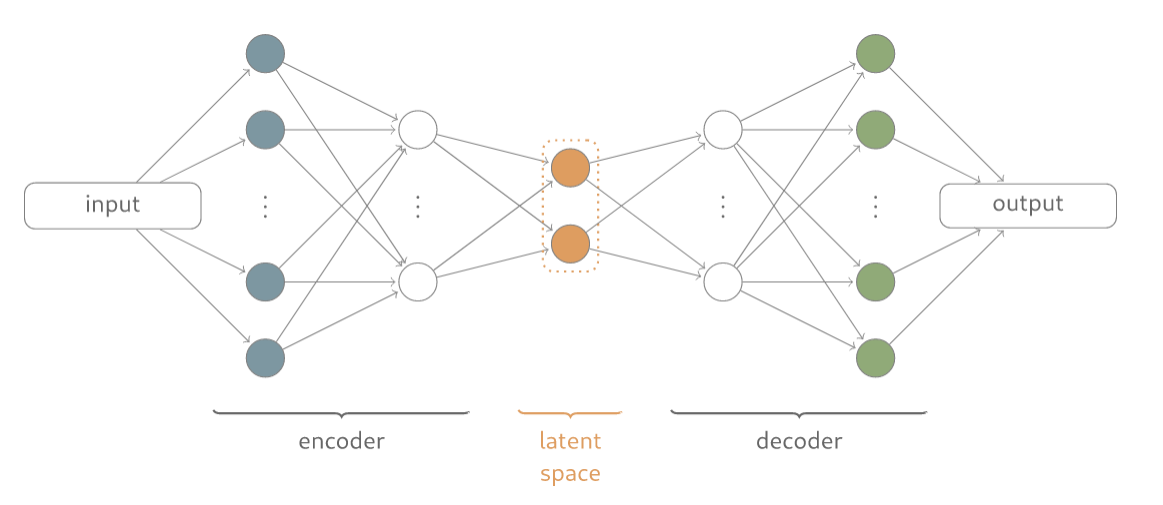
\includegraphics[width=1.0\textwidth,angle=0]{abb/ae_spinner}
    \caption[schematische Darstellung eines Autoencoders]{schematische Darstellung eines Autoencoders \cite{Spi2018}}
\end{figure}
Dies ist als eine Art Datenkompression zu sehen, da der Encoder spezifische Encodings generiert, die für die spätere Generierung der - dem orginalen Input sehr ähnlichen - Ausgabedaten nötig ist. Die Aufgabe des Encoders ist also, die Eingabedaten zu verarbeiten und sie einem Punkt im latenten Raum zuzuordnen. Als Verlustfunktion wird normalerweise entweder \frqq{mean-squared error\flqq} oder \frqq{cross-entropy\flqq} benutzt, um das Autoencoder-Netzwerk für Ausgaben zu bestrafen, die nicht den Eingaben entsprechen.
Da das Encoding bzw. der latente Raum sehr viel weniger Speicherplatz bedarf als die Originaleingabe, muss das Netzwerk Informationen verwerfen. Der Encoder lernt so viel wie nötig und so wenig wie möglich an relevanten Informationen im Encoding zu behalten, damit das Decodernetzwerk ein möglichst exaktes Abbild der Eingabedaten rekonstruieren kann \cite[S.64]{fos19}.
\begin{figure}[H]
    \centering
    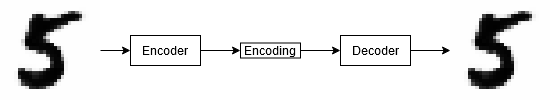
\includegraphics[width=1.0\textwidth,angle=0]{abb/autoencoder_standard}
    \caption[Autoencoder]{Funktionsweise eines Autoencoders am Beispielbild der Zahl \frqq{5\flqq} aus dem MNIST-Set}
\end{figure}
Standard-Autoencoder können also kompakte Datenrepräsentationen lernen und ihre Eingabedaten sehr gut rekonstruieren. Sie können auch sehr gut zur Bildreinigung verrauschter Bilder verwendet werden, da der Encoder lernt, dass die Position des Rauschens innerhalb des latenten Raums nicht relevant ist. Das Problem mit Standard-Autoencodern ist im Hinblick auf generative Modelle, dass sie keine Interpolation im latenten Raum zulassen \cite{Spi2018}. Man möchte ja mit generativen Modellen nicht die Originaldaten wiederherstellen, sondern dem latenten Raum zufällige Stichproben entnehmen bzw. Variationen der Eingabedaten aus dem latenten Raum generieren. Wenn diese Stichproben in Raumdiskontinuitäten liegen, werden inkorrekte Ausgabedaten erzeugt, weil der Decoder schlichtweg keine Erfahrung mit Datenpunkten aus dieser Region des latenten Raumes hat.

\subsubsection{VAE}~\\
Variational Autoencoder haben hingegen einen \emph{kontinuierlichen} latenten Raum, welcher eine Interpolation und zufällige Stichproben erlaubt.
\begin{figure}[H]
    \centering
    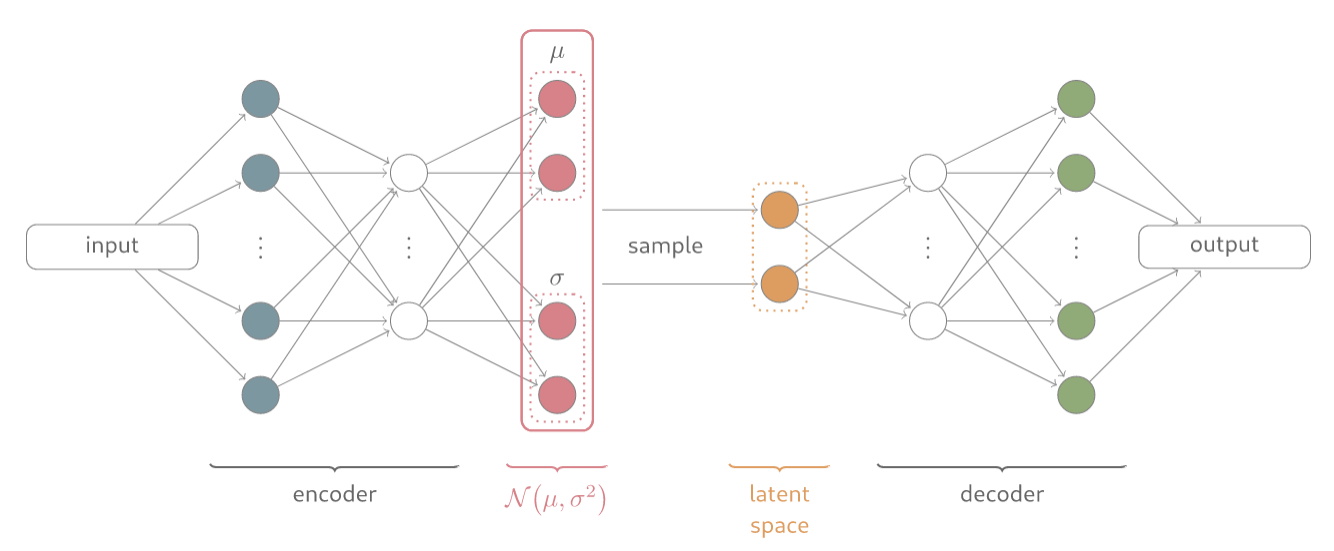
\includegraphics[width=1.0\textwidth,angle=0]{abb/vae_spinner}
    \caption[schematische Darstellung eines VAE]{schematische Darstellung eines VAE \cite{Spi2018}}
\end{figure}
Dies wird erreicht, indem der Encoder statt \emph{einem} Vektor der Größe $n$, \emph{zwei} Vektoren der Größe $n$ - $\mu$ und $\sigma$ - codiert. Dabei ist $\mu$ der Mittelwert der Verteilung und $\sigma$ der Logarithmus der Varianz jeder Dimension \cite{sha18}. In einem Standard-Autoencoder wird jedes Bild direkt auf einen Punkt im latenten Raum abgebildet. In einem VAE hingegen wird jedes Bild auf eine multivariate Normalverteilung um einen Punkt im latenten Raum abgebildet. Das bedeutet, dass der Encoder jede Eingabe zu einem Mittelwert- und einem Varianzvektor abbilden muss und sich nicht um die Kovarianz zwischen den Dimensionen zu sorgen braucht. Darüber hinaus ist $\sigma$ der Logarithmus der Varianz, da dieser eine beliebige reelle Zahl im Bereich ($-\infty, \infty$) annehmen kann, was dem natürlichen Ausgabebereich eines neuronalen Netzes entspricht, wohingegen die Varianz nur positive Werte annehmen kann \cite[S.81]{fos19}.
\begin{figure}[htb]
    \centering
    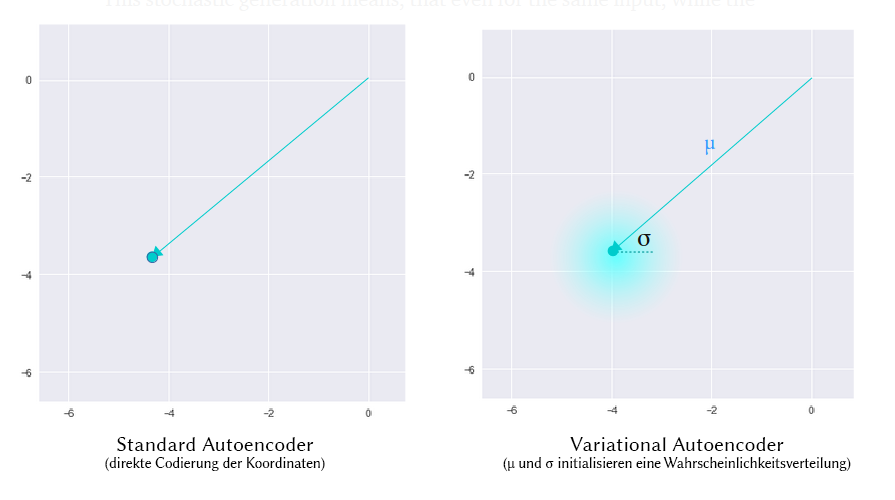
\includegraphics[width=0.9\textwidth,angle=0]{abb/VAE_muandsigma.png}
    \caption[Unterschied im Encoding - Autoencoder vs. VAE]{Unterschied im Encoding - Autoencoder vs. VAE \cite{sha18}}
\end{figure}
\FloatBarrier
Das Modell hat damit einen gewissen Grad an lokaler Variation im Encoding, jedoch keine überlappenden Cluster an variierenden Stichprobenencodings. Im Idealfall möchte man nicht nur im lokalen Stichprobenraum Variationen entnehmen, wo sich die Stichproben sehr ähnlich sind, sondern zwischen verschiedenen Klassen von Stichproben kontinuierlich interpolieren. Alle erkannten Merkmalcluster sollen also so nah wie möglich aneinander im latenten Raum angeordnet sein. Dies wird mit der Einrechnung der Kullback-Leibler-Divergenz in die Verlustfunktion erreicht \cite{sha18}. Die KL-Divergenz ist eine Methode, um zu messen, wie sehr sich eine Wahrscheinlichkeitsverteilung von einer anderen unterscheidet. Im Fall eines VAE soll gemessen werden, wie sehr sich die Normalverteilung mit den Parametern $\mu$ und $\sigma$ von der Standardnormalverteilung (Glockenkurve) unterscheidet. Das Netzwerk wird damit für die Codierung von Beobachtungen zu $\mu$ und $\sigma$ bestraft, die deutlich unterschiedlich von den Parametern einer Standardnormalverteilung sind \cite[S.102]{fos19}.
\begin{figure}[H]
    \centering
    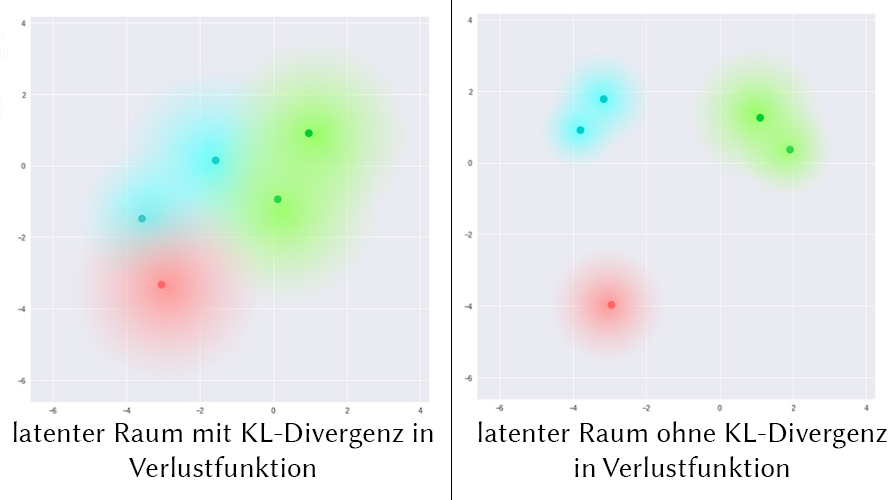
\includegraphics[width=0.7\textwidth,angle=0]{abb/VAE_KLL}
    \caption[Verteilung der Cluster mit und ohne KL-Divergenz]{Verteilung der Cluster mit und ohne KL-Divergenz \cite{sha18}}
\end{figure}
Mit einer optimierten Verlustfunktion und der KL-Divergenz können Verteilungen wie in Abbildung 2.6 erreicht werden.
\begin{figure}[H]
    \centering
    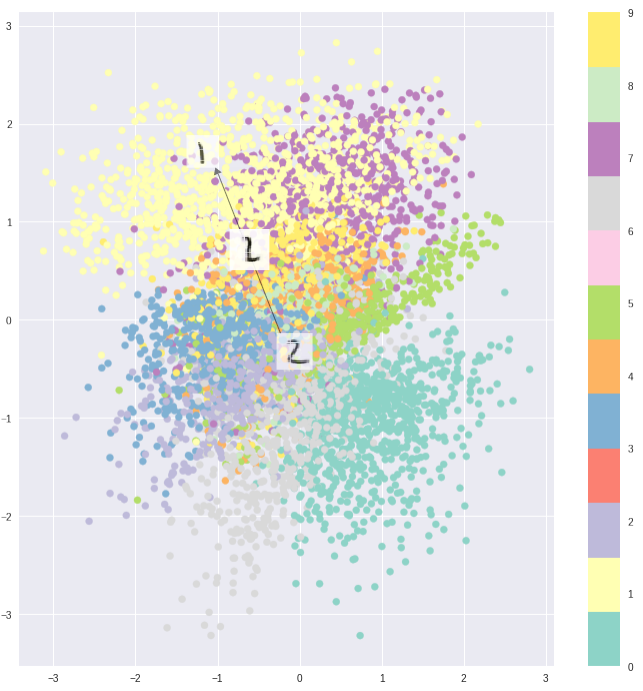
\includegraphics[width=0.6\textwidth,angle=0]{abb/vae_final.png}
    \caption[Verteilung im Encoding eines VAE]{Verteilung im Encoding eines VAE am Beispiel des MNIST-Sets \cite{sha18}}
\end{figure}


\subsection{Generative Adversarial Networks (GANs)}\label{Generative Adversarial Networks (GANs)}

Die GAN-Architektur für ein auf Deep Learning basierendes, generatives Modell wurde erstmals 2014 von Ian Goodfellow, et al. auf der NIPS-Konferenz vorgestellt. Sie besteht aus zwei Submodellen:
\begin{itemize}
    \item Generator (G) - Modell, das neue Beobachtungen als Eingabedaten generiert
    \item Diskriminator (D) - Modell, das klassifiziert, ob die zugeführten Daten vom Trainingset oder vom Generator stammen
\end{itemize}
Beide Modelle werden gleichzeitig trainiert. Der Generator versucht, Zufallsrauschen in Beobachtungen umzuwandeln, die so aussehen, als würden sie dem Trainingsdatensatz entstammen, und der Diskriminator versucht zu erkennen, ob eine Beobachtung aus dem ursprünglichen Datensatz stammt oder eine der Fälschungen des Generators ist \cite{bro19}. Am Anfang gibt der Generator sehr verrauschte Bilder aus und der Diskriminator prognostiziert zufällig. Der entscheidende Punkt von GANs ist, wie das Training der beiden Netzwerke abgewechselt wird, sodass, sobald der Generator geschickter im Täuschen des Diskriminators wird, dieser sich anpassen muss, um weiterhin die gefälschten Bilder zu erkennen. Das wiederum treibt den Generator dazu an, neue Wege zu finden, um den Diskriminator zu täuschen \cite[S.99]{fos19}.
\begin{figure}[H]
    \centering
    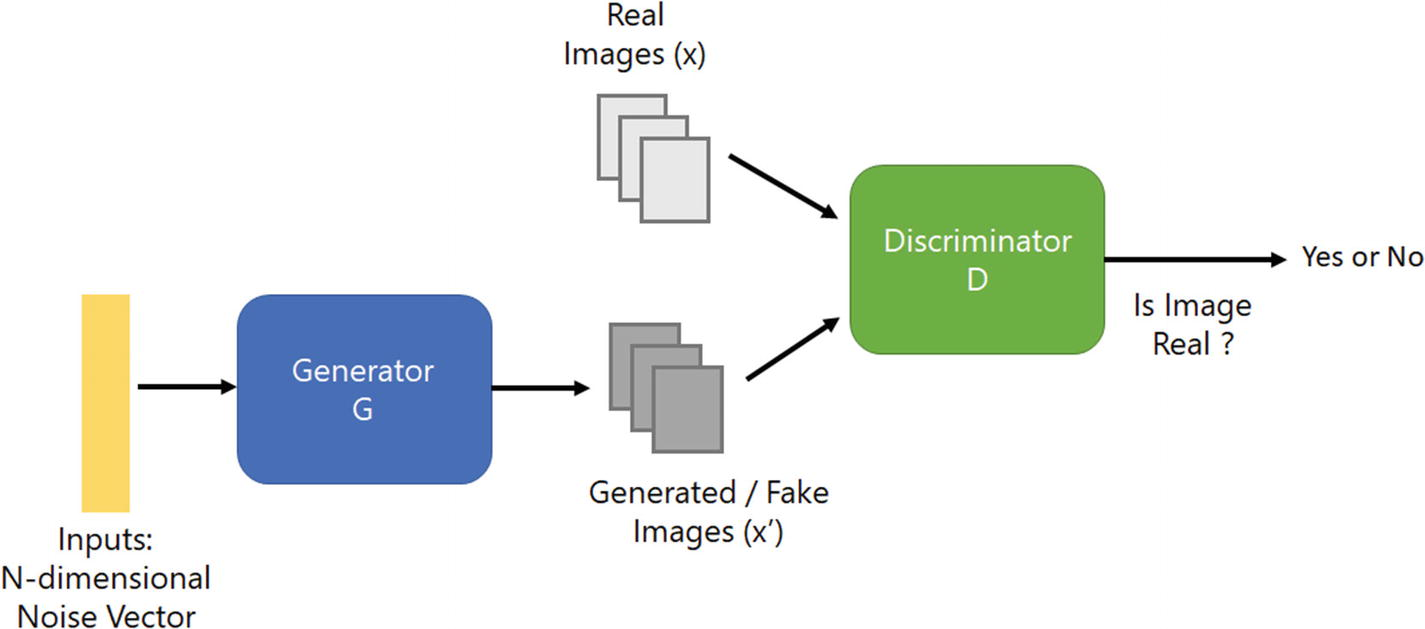
\includegraphics[width=1\textwidth,angle=0]{abb/Springer_GAN}
    \caption[Funktionsweise eines GAN]{Funktionsweise eines GAN \cite{SDT18}}
\end{figure}
Man kann sich das Training eines GAN als Nullsummenspiel vorstellen: "Das Generatornetzwerk sei dabei ein Geldfälscher, der versucht, Falschgeld zu produzieren. Das Diskriminatornetzwerk sei die Polizei, die versucht, echtes Geld von gefälschtem Geld zu unterscheiden. Um das Spiel zu gewinnen muss, der Geldfälscher lernen, Geldscheine zu erzeugen, welche von echtem Geld ununterscheidbar sind." \cite{goo16} In diesem Fall bedeutet Nullsummenspiel, dass das jeweilige Netzwerk per Fehlerrückführung in jedem Trainingsschritt bestraft wird und dessen Modellparameter variiert werden. So entsteht nach sehr vielen Trainingsschritten ein generatives Modell, welches täuschend echte Daten generieren kann. Die GAN-Architektur wird vor allem bei der Generierung von Bilddaten verwendet.

Im Original-GAN-Forschungspaper wurden dichte Schichten anstelle der Konvolutionsschichten für das Training verwendet. Seitdem hat sich jedoch gezeigt, dass Konvolutionsschichten dem Diskriminator eine bessere Vorhersagekraft verleihen. Diese Art von GANs wird in der Literatur auch DCGAN (Deep Convolutional Generative Adversarial Network) genannt, aber heutzutage enthalten fast alle GAN-Architekturen Konvolutionsschichten, sodass das »DC« bereits enthalten ist, wenn über GANs geredet wird \cite{bro19}. Seit der ersten Vorstellung 2014 wurden bis heute mehr als 500 verschiedene Erweiterungen von GAN-Architekturen in wissenschaftlichen Papers vorgestellt. Diese haben dann spezielle Eigenschaften, die zu einer verbesserten Lösung der jeweiligen Aufgabenstellung führt.
